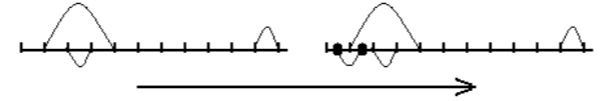
\includegraphics[scale=0.8]{teleport.png}

The first figure shows a segment with the three original teleporters. The second figure shows the same segment after adding a new teleporter with endpoints at 0.5 and at 1.5. 

In first example, after adding the new teleporter as shown in the figure, your travel would be the following:
\begin{itemize}
\item You start at position 0, moving eastward.
\item You reach the endpoint at position 0.5 and get teleported to position 1.5 (you earn 1 point).
\item You continue to move east and reach endpoint at position 2; you get teleported to position 3 (you have 2 points).
\item You reach endpoint at position 4, and get teleported to 1 (you have 3 points).
\item You reach endpoint at 1.5, and get teleported to 0.5 (you have 4 points).
\item You reach endpoint at 1, and get teleported to 4 (you have 5 points).
\item You reach endpoint at 10, and get teleported to 11 (you have 6 points).
\item You continue until you reach the end of the segment finishing with a total score of 6 points.
\end{itemize}